%=====================================================================
%  A Certified Indistinguishability Floor and Safe Discrimination
%  Beyond Classical Waveforms in a Caputo Strong-Allee Predator-Prey Model
%
%  Native LaTeX. Compiles with pdflatex + bibtex-free thebibliography,
%  no shell-escape, no non-standard packages.
%=====================================================================
\documentclass[mathematics,article,accept,pdftex,moreauthors]{Definitions/mdpi}

\usepackage{amsmath,amssymb,amsthm}
\usepackage[none]{hyphenat}

\DeclareMathOperator{\Real}{Re}
\DeclareMathOperator{\Imag}{Im}
\newcommand{\Dc}[1]{{}^{C}\!D^{#1}}
\newcommand{\Estate}{\widehat{E}_m^{\mathrm{state}}}

\firstpage{1}
\makeatletter
\setcounter{page}{\@firstpage}
\makeatother
\pubvolume{1}
\issuenum{1}
\articlenumber{0}
\pubyear{2026}
\copyrightyear{2026}
\externaleditor{ }
\datereceived{ }
\dateaccepted{ }
\datepublished{ }
\hreflink{https://doi.org/}

\Title{A Certified Indistinguishability Floor and Safe Discrimination Beyond Classical Waveforms in a Caputo Strong-Allee Predator--Prey Model}

\Author{{Ibrahim Alraddadi} $^{1,*}$}

\AuthorNames{Ibrahim Alraddadi}

\address{%
$^{1}$ \quad Department of Mathematics, Faculty of Science, Islamic University of Madinah, Madinah, {42351}, Saudi Arabia}

\corres{Correspondence: ialraddadi@iu.edu.sa}

\abstract{A fitted fractional order does not identify a fractional mechanism: on a finite horizon, delayed feedback or a few hidden states reproduce similar trajectories. For a strong-Allee predator--prey system with locked ecology, we quantify when a controlled experiment can separate Caputo, delayed, integer-order, and finite-latent response laws while keeping the prey above its Allee threshold. The first main result is a certified indistinguishability floor: for the linearized prey response, an exact two-point minimax bound, uniform over every input in the declared budget, is combined with interval-certified $L^{1}$ approximation errors of finite-state surrogates. A partial-fraction reduction eliminates the stiffness of surrogates whose rates span forty-one orders of magnitude, and interval Newton certifies all surrogate poles, giving $\|g_\alpha-g_m\|_{L^1}\le 4.9\cdot10^{-5}$ and a certified floor above $0.49998$ at latent order $m=128$: at attainable latent orders the finite-state rival cannot be distinguished, for any admissible input. The second main result is empirical and points the other way. Among six classical excitation families the accuracy-leading inputs all cross the Allee threshold, suggesting an intrinsic safety--informativeness frontier; a constrained search over $163{,}840$ waveforms at the same amplitude budget refutes that reading, returning piecewise-constant designs with four-class model-selection accuracy $0.803$ and no observed crossings, against $0.514$ for the only safe classical family. Safety of the leading designs is verified a posteriori, with validated enclosures for four of eight headline trajectories. An empirically anchored vole--weasel case study in a fractional-stabilization regime reproduces the structure of both results and predicts that gestation delays are practically unidentifiable at saturated predation. Identifying ecological memory is therefore limited by the declared rival-complexity budget, not by the safety margin.}

\keyword{Caputo fractional derivative; strong Allee effect; model discrimination; optimal experimental design; time-delay systems; certified interval arithmetic; Mittag-Leffler functions; safe excitation}

\MSC{34A08; 34K20; 62K05; 92D25; 65G20}

\begin{document}

%=====================================================================
\section{Introduction}
\label{sec:intro}

Caputo derivatives of order $0<\alpha<1$ model hereditary effects in viscoelasticity, anomalous transport, and population dynamics \cite{Podlubny1999,Diethelm2010,Kilbas2006,Mainardi2010}, and fractional predator--prey models form a sizeable literature \cite{Ahmed2007,Javidi2013,Vargas2015,Rihan2021}. Underneath this literature sits an identification problem. Estimating $\alpha<1$ from data does not establish a fractional mechanism, because on a bounded window $[0,T]$ a delay term $\xi(t-\tau)$ or a low-dimensional latent state $q\in\mathbb{R}^{m}$ generates trajectories within the noise floor of the fractional ones; Corollary~\ref{cor:closure} below makes this quantitative. Design methods for fractional-order \emph{estimation} exist \cite{FOED1,FOED2,FOED3}, and safety-constrained information acquisition has been analyzed in general settings \cite{Saligrama2026,Ni2026}. The intersection studied here is discrimination between memory \emph{mechanisms} under an ecological safety constraint:

\begin{quote}
\emph{Which perturbations and measurements can distinguish fractional memory from delayed or latent alternatives in a strong-Allee ecological system, and when does ecological safety make that discrimination fundamentally difficult?}
\end{quote}

Safety is not decorative in this question. Below the Allee threshold $A$, the prey growth term $P(x)=rx(1-x/K)(x/A-1)$ turns negative and collapse is irreversible, so the perturbations most informative about memory---peak amplitudes near the budget, broadband spectra---are the ones most likely to destroy the object of study. Among six classical excitation families, the best-discriminating input crosses the threshold in $100\%$ of stable-regime benchmark cells (Section~\ref{sec:safe}), which suggests that safety and informativeness are in intrinsic conflict. One of the two principal findings of this paper is that this suggestion is wrong: the severe frontier is a property of the waveform parameterization, not of the system.

The ecological backbone follows the companion certification study \cite{Companion}: the equations, the locked parameters, the coexistence equilibrium, and the Jacobian are restated below for completeness and are not claimed as contributions. That study certifies dynamical regimes of a specified Caputo model; it does not address whether such a model can be told apart from a delayed or latent mechanism reproducing the same observations to within the noise level $\sigma$, which is the question posed here. No result below recertifies the backbone. With the ecology frozen, any difference between simulated observations is attributable to the memory law or to the experiment, never to an altered population model.

\subsection*{Related Work and What Is New Here}

We do not claim novelty for the strong-Allee backbone or its stability geometry \cite{Companion}, for the structural separation of fractional transfers from rational and retarded-delay ones (classical branch-point material \cite{Matignon1996,Petras2011}), for positive exponential-sum approximation of the fractional kernel---the construction, the positivity of the weights, and the root-exponential order are due to McLean \cite{McLean2018}, building on Beylkin and Monz\'on \cite{Beylkin2005,Beylkin2010} and underlying fast Caputo evaluation \cite{Jiang2017}---for the analytic-strip trapezoidal estimate \cite{Trefethen2014}, for two-point Gaussian testing bounds \cite{Kay1998}, or for safe experimental design as a general theory \cite{Saligrama2026,Ni2026}. The new content is the following, with the evidence class of each item stated using the labels \emph{theorem} (analytic proof), \emph{certified} (rigorous interval enclosure with outward rounding), and \emph{corroboration} (floating-point experiment).

\begin{enumerate}
\item \textbf{A certified indistinguishability floor at the response level (theorem + certified).} An exact two-point minimax bound (Theorem~\ref{thm:floor}), routed through the $L^{1}$ norm of the response kernel and therefore uniform over every admissible input, is combined with interval-certified surrogate errors: an optimized finite-state class up to $m=32$, and an explicit positive-exponential-sum surrogate up to $m=128$ via a partial-fraction reduction and interval-Newton pole certification (Section~\ref{sec:floor}). The certified floor exceeds $0.49998$ at $m=128$.
\item \textbf{An endpoint-inclusive approximation lemma with exact horizon scaling (structural lemma, attributed technique).} The published exponential-sum estimates exclude the kernel singularity at $t=0$; Lemma~\ref{lem:soe} records an $L^{1}(0,T)$ form including the endpoint, with the exact scaling $E^{+}_{m}(\alpha,T)=T^{\alpha}E^{+}_{m}(\alpha,1)$ and rate $e^{-c\sqrt{m}}$ for every $c<\pi\sqrt{\alpha(1-\alpha)}$.
\item \textbf{Refutation of the classical safety--informativeness frontier (corroboration, with certified safety elements).} A constrained search over $163{,}840$ candidate waveforms at a fixed peak budget and hard Allee margin returns piecewise-constant designs that are simultaneously safe and more informative than every classical family, safe or not ($0.803$ versus $0.514$ for the only safe classical family and $0.763$ for the best classical design of any kind); a held-out control shows the advantage is not an in-sample artifact (Section~\ref{sec:safe}).
\item \textbf{Trajectory safety with stated rigor (certified + corroboration).} Safety of the headline designs is verified a posteriori by mesh refinement with a rigorous inter-node modulus bound; for four of the eight headline trajectories a validated enclosure with self-consistent error control is obtained, and only those are called rigorous. Interval-certified constants show that the invariant-ball route to nonlinear safety admits inputs seventy times smaller than the amplitude actually used, closing that route (Section~\ref{sec:safety-status}).
\item \textbf{An empirically anchored case study (corroboration + certified).} The vole--weasel instantiation of Section~\ref{sec:case} re-runs the full pipeline at a literature-anchored operating point in the fractional-stabilization regime: the certified floor persists ($0.4999992$ at $m=128$), safety rankings invert while the worst-case criterion and the transferred searched design survive, and functional-response saturation renders the delayed mechanism unidentifiable.
\item \textbf{A reproducibility control (corroboration).} The frozen four-class benchmark reproduces to four decimal places on an independent host under a re-implemented driver and different library versions (Section~\ref{sec:numerics}).
\end{enumerate}

Items 1--2 identify the obstruction that binds; items 3--4 show that the obstruction commonly blamed---safety---does not. The paper is organized so that every claim carries its evidence class, boundary cases are stated, and the scope of each statement is fixed by an explicit proposition (Proposition~\ref{prop:scope}).

%=====================================================================
\section{Model, Response Classes, and Observation Protocol}
\label{sec:model}

\subsection{The Locked Ecology and the Four Response Laws}

The backbone is the planar strong-Allee predator--prey field
\begin{equation}
f(x,y)=\begin{pmatrix} r x\left(1-\dfrac{x}{K}\right)\left(\dfrac{x}{A}-1\right)-\dfrac{a x y}{1+h x}\\[2mm]
\dfrac{e a x y}{1+h x}-\mu y\end{pmatrix},
\label{eq:field}
\end{equation}
with the parameters locked at the exact rationals $(r,K,a,h,e,\mu)=(\tfrac32,1,1,\tfrac12,\tfrac45,\tfrac25)$ of \cite{Companion}, chosen there for exact arithmetic; they are an instance, not a calibration, and no empirical meaning is attached to them (Section~\ref{sec:discussion}). The coexistence equilibrium is $x^{*}=2/3$, $y^{*}(A)=2(2-3A)/(9A)$, and the Jacobian $J(A)$ at the equilibrium has $\operatorname{tr}J=(7A-2)/(8A)$ and $\det J=(2-3A)/(20A)$, both exact; at the benchmark threshold $A=1/4$,
\begin{equation}
J=\begin{pmatrix}-1/8 & -1/2\\ 1/2 & 0\end{pmatrix},\qquad \operatorname{tr}J=-\tfrac18,\qquad \det J=\tfrac14 .
\label{eq:J}
\end{equation}
Stability of the Caputo equilibrium across $(A,\alpha)$, including the Matignon boundary $\alpha^{*}(A)$, is certified in \cite{Companion} and used here only to select admissible operating regimes.

Four response laws compete on this fixed ecology, differing only in the memory mechanism: the integer-order law $\dot z=f(z)+Bu$; the Caputo law $\Dc{\alpha}z=f(z)+Bu$ with $\alpha\in(0,1)$; a retarded delay law in which the trophic gain acts through $x(t-\tau)$ with gestation delay $\tau=0.35$; and a latent law $\dot z=f(z)+g\mathbf{1}^{\top}q+Bu$, $\dot q=-\Lambda q+\mathbf{1}u$ with $m$ relaxation modes, rates $\Lambda=\operatorname{diag}(0.6,1.0,0.4)$ and coupling $g=0.15$ in the benchmark. The input enters the prey channel, $B=e_{1}$, with peak budget $\|u\|_\infty\le0.10$; observations are $y_k=Cz(t_k)+\varepsilon_k$ on prey, predator, or both, with i.i.d.\ Gaussian noise of level $\sigma$. The delay and latent rivals are calibrated alternative response laws matched at the same operating point, channel, and units; only the integer and Caputo laws share $J(A)$ exactly.

\begin{figure}[H]
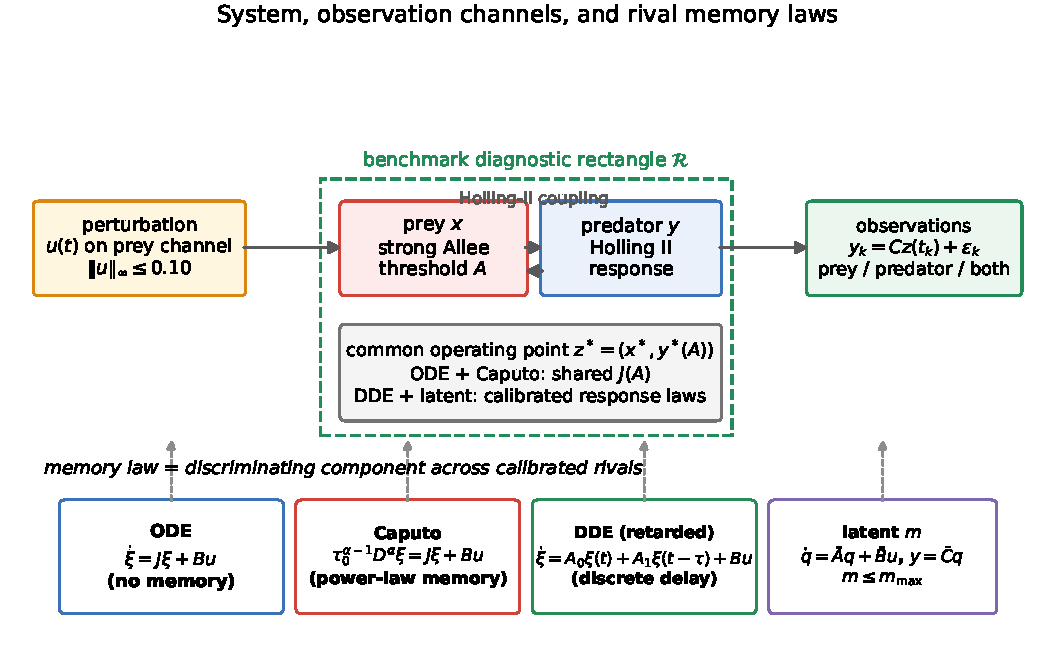
\includegraphics[width=0.8\textwidth]{fig11_system_schematic.pdf}
\caption{The discrimination setting (exposition): one locked strong-Allee ecology \eqref{eq:field}, four competing memory mechanisms differing only in the response law, a prey-channel perturbation $u$ with peak budget $\|u\|_{\infty}\le0.10$, and noisy observations on prey, predator, or both. The experiment must separate the mechanisms without driving the prey below the Allee threshold $A$.}
\label{fig:schematic}
\end{figure}

\subsection{Solution Concept and Well-Posedness}

For the Caputo law we work with mild solutions of the Volterra form $z(t)=z_{0}+\Gamma(\alpha)^{-1}\int_{0}^{t}(t-s)^{\alpha-1}\left[f(z(s))+Bu(s)\right]ds$; the field \eqref{eq:field} is locally Lipschitz on the open positive quadrant away from the singular line $1+hx=0$, so local existence and uniqueness for continuous inputs follow from the standard fractional Picard theory \cite{Diethelm2010,Kilbas2006}, and positivity, a uniform ultimate bound, and global continuation on the regimes used here are proved in \cite{Companion}; we do not repeat those arguments and we use trajectories only on windows where they apply. The linearized analysis of Sections~\ref{sec:sep} and \ref{sec:floor} concerns the transfer operator of the linearization at the coexistence equilibrium and requires no nonlinear continuation. All benchmark trajectories are additionally screened for divergence, and none occurs in any experiment reported below.

\subsection{Safety}

An experiment is \emph{safe} on a trajectory when $\min_{t\in[0,T]}x(t)>A$: the prey never enters the irreversible collapse region. Throughout, $T=12$ and the benchmark grid uses $A\in\{0.20,0.25\}$ for the stable-regime task. Since the true mechanism is unknown to the experimenter, a design is called safe only when it is safe under \emph{all four} candidate laws; Section~\ref{sec:safety-status} states the exact rigor of each safety verdict.

%=====================================================================
\section{Exact Separation and Finite-Horizon Approximation}
\label{sec:sep}

This section fixes the analytic geometry of the discrimination problem: the mechanisms are exactly separated in the frequency domain, yet finite-horizon approximation closes the gap at finite latent order. Both facts are needed to read the floor of Section~\ref{sec:floor} correctly.

\subsection{Structural Separation}

Write $G_{\alpha}(s)=C\left(s^{\alpha}I-J\right)^{-1}B$ for the transfer of the linearized Caputo law on the prey channel ($C=B^{\top}=e_{1}^{\top}$).

\begin{Theorem}[structural separation; classical mechanism, stated for scope]
\label{thm:sep}
Let $CB\neq0$ and $\alpha\in(0,1)$ be irrational. Then $G_{\alpha}$ is not meromorphic in any neighborhood of $s=0$; in particular it differs, as a function on any open frequency set, from every finite-dimensional rational transfer and from every strictly proper retarded-delay transfer. At high frequency $|G_{\alpha}(i\omega)|=O(\omega^{-\alpha})$, a decay no rational transfer (integer rolloff) and no strictly proper retarded transfer ($O(\omega^{-1})$) reproduces exactly.
\end{Theorem}

The mechanism---a branch point of $s^{\alpha}$ at the origin against the meromorphy of the rival classes---is classical \cite{Matignon1996,Petras2011}, and no priority is claimed. Figure~\ref{fig:transfer} displays the magnitude and phase signatures on the benchmark. The statement concerns exact equality of transfers; it promises nothing about experiments with finite bandwidth, horizon, and noise. That regime is governed by the following lemma.

\begin{figure}[H]
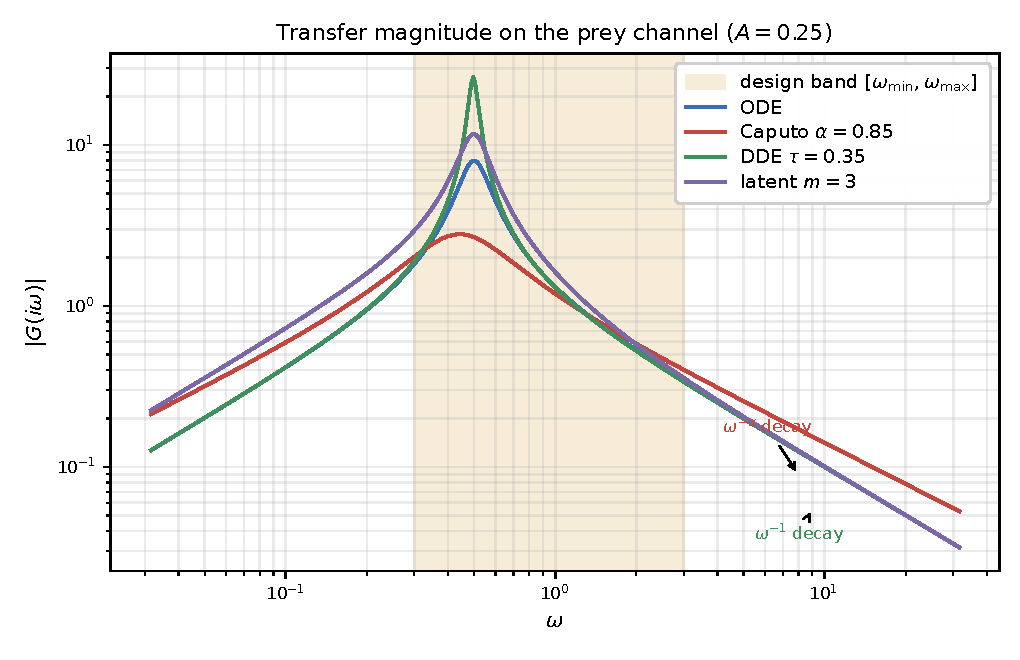
\includegraphics[width=0.48\textwidth]{fig01_transfer_magnitude.pdf}
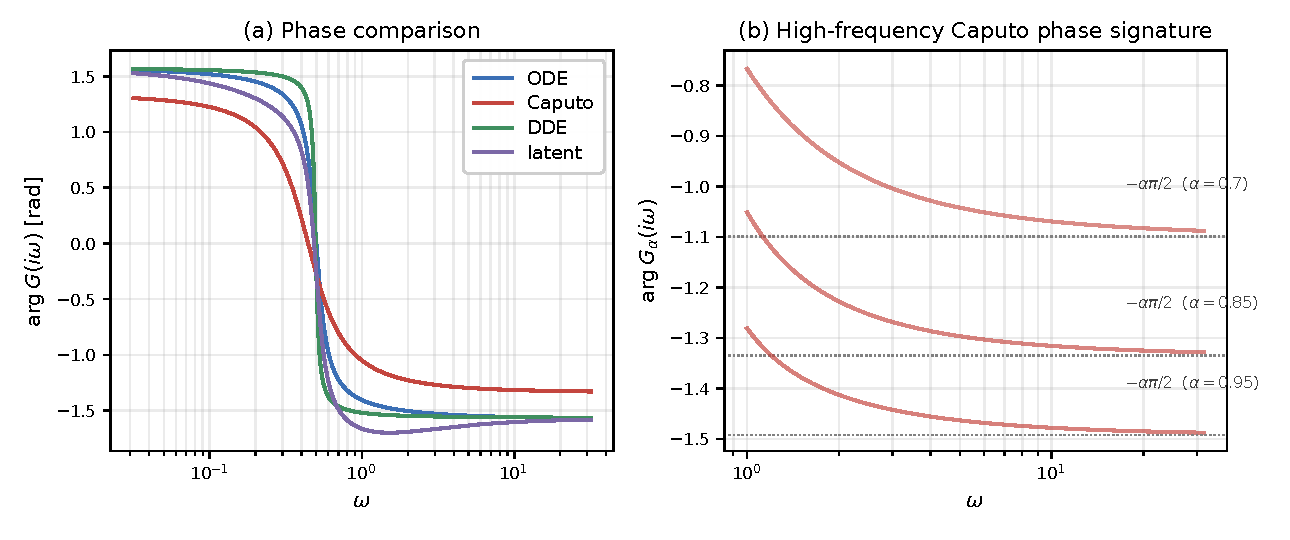
\includegraphics[width=0.48\textwidth]{fig02_phase_2panel.pdf}
\caption{Frequency signatures of the four linearized response laws on the benchmark (analytic content; curves are exact transfer evaluations, not simulations). Left: magnitude, with the $O(\omega^{-\alpha})$ fractional rolloff separating the Caputo law from the integer ($\omega^{-1}$-type) decays. Right: phase, where the fractional law approaches $-\alpha\pi/2$ while rational rivals approach integer multiples of $-\pi/2$. Exact separation (Theorem~\ref{thm:sep}) coexists with finite-horizon mimicry (Corollary~\ref{cor:closure}); the remainder of the paper quantifies the tension.}
\label{fig:transfer}
\end{figure}

\subsection{An Endpoint-Inclusive Positive Exponential-Sum Estimate}

The Caputo kernel $k_{\alpha}(t)=t^{\alpha-1}/\Gamma(\alpha)$ has the Stieltjes representation $k_{\alpha}(t)=c_{\alpha}\int_{0}^{\infty}\lambda^{-\alpha}e^{-\lambda t}\,d\lambda$ with $c_{\alpha}=\sin(\pi\alpha)/\pi$. Discretizing by the trapezoidal rule on a logarithmic grid $\lambda_{k}=e^{kh}$ and truncating produces an exponential sum with \emph{positive} weights and rates. This construction, including the positivity and the root-exponential order, is due to McLean \cite{McLean2018}, building on \cite{Beylkin2005,Beylkin2010}, and underlies fast Caputo evaluation \cite{Jiang2017}; the quadrature estimate invoked below is the analytic-strip trapezoidal bound \cite{Trefethen2014}, and root-exponential order is the expected optimal order for an algebraic branch point \cite{Stahl2003}. We claim no new approximation method, no new rate law, and no priority for positive weights. What we add is narrow: the published estimates are stated on compact intervals $[\delta,T]$, $\delta>0$, excluding the singularity, whereas the convolution argument of Section~\ref{sec:floor} needs the $L^{1}(0,T)$ norm \emph{including} $t=0$.

\begin{Lemma}[endpoint-inclusive $L^{1}$ estimate and exact horizon scaling]
\label{lem:soe}
Let $E^{+}_{m}(\alpha,T)$ denote the least $L^{1}(0,T)$ error of an $m$-term exponential sum with positive weights and rates. Then
\begin{equation}
E^{+}_{m}(\alpha,T)=T^{\alpha}\,E^{+}_{m}(\alpha,1),
\label{eq:scaling}
\end{equation}
and for every $c<\pi\sqrt{\alpha(1-\alpha)}$ there exists $A(\alpha,c)<\infty$ with
\begin{equation}
E^{+}_{m}(\alpha,T)\le A(\alpha,c)\,T^{\alpha}e^{-c\sqrt{m}}\qquad(m\ge1).
\label{eq:rootexp}
\end{equation}
Consequently $m(\varepsilon)=O\!\left(\log^{2}(1/\varepsilon)\right)$ terms suffice for accuracy $\varepsilon$.
\end{Lemma}

\begin{proof}
Equation \eqref{eq:scaling} is exact: substituting $t=Ts$ and using $k_{\alpha}(Ts)=T^{\alpha-1}k_{\alpha}(s)$ turns the $L^{1}(0,T)$ error into $T^{\alpha}$ times the $L^{1}(0,1)$ error, and $(c_{j},\lambda_{j})\mapsto(T^{1-\alpha}c_{j},T\lambda_{j})$ is a bijection of the admissible positive mixtures, so the infima coincide. For \eqref{eq:rootexp}, put $\lambda=e^{x}$, so $k_{\alpha}(t)=c_{\alpha}\int_{\mathbb{R}}g(x,t)\,dx$ with $g(x,t)=e^{(1-\alpha)x}e^{-te^{x}}$. For $|\Imag x|\le d<\pi/2$ one has $|g|\le e^{(1-\alpha)\Real x}e^{-te^{\Real x}\cos d}$, whence the strip norm obeys $N(g(\cdot,t),d)\le 2(\cos d)^{\alpha-1}\Gamma(1-\alpha)t^{\alpha-1}$; this bound is $t$-integrable on $(0,1)$ because $\alpha>0$, so no excision of the endpoint is required. Integrating the trapezoidal estimate of \cite{Trefethen2014} over $t\in(0,1)$ and using $\int_{0}^{1}t^{\alpha-1}dt=1/\alpha$ with $c_{\alpha}\Gamma(1-\alpha)=1/\Gamma(\alpha)$ bounds the discretization error by $2\,\Gamma(\alpha+1)^{-1}(\cos d)^{\alpha-1}e^{-2\pi d/h}(1-e^{-2\pi d/h})^{-1}$; the truncation tails contribute $O(e^{-\alpha M_{+}h})$ and $O(e^{-(1-\alpha)M_{-}h})$. Equalizing the three exponents gives $m\approx 2\pi d\,h^{-2}[\alpha(1-\alpha)]^{-1}$ and exponent $\sqrt{2\pi d\,\alpha(1-\alpha)m}$, which tends to $\pi\sqrt{\alpha(1-\alpha)m}$ as $d\uparrow\pi/2$ while $(\cos d)^{\alpha-1}\to\infty$. Hence any $c$ strictly below the limit is attained with a finite constant.
\end{proof}

The quantifier order is not cosmetic: the constant diverges as $c\uparrow\pi\sqrt{\alpha(1-\alpha)}$, so the boundary rate is \emph{not} established here, and whether it is attained or optimal is open. Equation \eqref{eq:scaling} is verified to machine precision over a $285$-cell sweep ($\alpha\in\{0.30,\dots,0.95\}$, $T\in\{1,10,100\}$, $m\le128$): the measured ratio $E(T)/E(1)$ equals $T^{\alpha}$ to all printed digits. Over the same sweep, \eqref{eq:rootexp} holds at $c=\pi\sqrt{\alpha(1-\alpha)}$ with constants between $0.29$ and $11.1$ and is attained to within a factor $1.00$ at $\alpha=0.70$, $m=128$ (corroboration, not part of the proof).

\begin{Corollary}[finite-horizon closure of the latent hierarchy]
\label{cor:closure}
For every $T<\infty$ and $\varepsilon>0$, some finite positive exponential mixture lies within $\varepsilon$ of $k_{\alpha}$ in $L^{1}(0,T)$. Hence, absent a declared bound on the latent dimension, no fixed finite-horizon experiment can guarantee a uniform positive separation from the whole latent hierarchy: discrimination is meaningful only relative to a budget $m$.
\end{Corollary}

\subsection{Three Error Objects}
\label{sec:semantics}

Three quantities recur and are never interchanged: (O1) the \emph{memory-kernel error} $\|k_{\alpha}-k_{m}\|_{L^{1}(0,T)}$, a statement about the fractional operator alone; (O2) the \emph{induced response error} $\|g_{\alpha}-g_{m}\|_{L^{1}(0,T)}$ between impulse responses of the linearized plant, equal to the $L^{\infty}\!\to\!L^{\infty}$ operator norm of the difference of input--output maps; and (O3) the \emph{fixed-input discrepancy} $\|(g_{\alpha}-g_{m})*u\|/\|u\|$ for one specific $u$. By construction $\mathrm{(O3)}\le\mathrm{(O2)}$ for every admissible $u$, but no constant relates (O1) to (O2): computed from the same surrogate family, the plant \emph{attenuates} the kernel error monotonically, by a factor $1.009$ at $m\approx5$ falling to $0.675$ at $m=128$. Kernel-level numbers are therefore never propagated into response-level claims in this paper. Because (O2) is a supremum over inputs, the floor of Section~\ref{sec:floor} is uniform over the admissible input class; for the same reason, (O2) is an \emph{obstruction certificate and not a design objective}---the frequency band maximizing $|G_{\alpha}-G_{m}|$ selects the multiscale waveform, which excites $87\%$ of the worst case at $m=32$ yet is the \emph{least} informative design in the four-class benchmark of Section~\ref{sec:safe}. Maximizing one pairwise discrepancy does not maximize multi-class accuracy.

%=====================================================================
\section{A Certified Indistinguishability Floor}
\label{sec:floor}

The first principal result combines an exact minimax bound with interval-certified approximation errors. The outcome is a floor on the error of \emph{any} test between the fractional response and a finite-latent rival that holds uniformly over every input in the budget, with every constant either exact or an outward-rounded enclosure.

\subsection{The Exact Two-Point Bound}

Fix the observation model: the prey channel is sampled at times in $(0,T]$ and corrupted by additive Gaussian noise with common covariance $\sigma^{2}I$ under both hypotheses. The hypotheses are ``the response kernel is $g_{\alpha}$'' and ``the response kernel is $g_{m}$'', with means obtained by convolving the respective kernels with the same admissible input $u$.

\begin{Theorem}[exact two-point floor under a response budget]
\label{thm:floor}
Let $\|u\|_{2}\le B$ and $d=\|\mu_{\alpha}-\mu_{m}\|_{2}/\sigma$. The minimax error of any test between the two hypotheses equals $P_{e}^{*}=\Phi(-d/2)$, and Young's inequality $\|(g_{\alpha}-g_{m})*u\|_{2}\le\|g_{\alpha}-g_{m}\|_{L^{1}}\|u\|_{2}$ gives
\begin{equation}
P_{e}^{*}\;\ge\;\Phi\!\left(-\frac{\Estate B}{2\sigma}\right)\;\longrightarrow\;\tfrac12
\qquad\text{as }\Estate\to0\text{ with }B,\sigma\text{ fixed,}
\label{eq:floor}
\end{equation}
where $\Estate$ is any upper bound on $\|g_{\alpha}-g_{m}\|_{L^{1}(0,T)}$. The bound is uniform over all $u$ with $\|u\|_{2}\le B$ and over any sampling schedule in $(0,T]$.
\end{Theorem}

The two-point Gaussian identity is textbook \cite{Kay1998}; the content is the pairing with a \emph{certified} $\Estate$ at the response level, never through $\|k_{\alpha}-k_{m}\|_{L^{2}}$, which is infinite for $\alpha\le1/2$ and would make such a statement vacuous on part of the declared range. Equality cases are transparent: \eqref{eq:floor} is an equality exactly when $u$ attains the Young bound, and the floor degenerates to the trivial $P_{e}^{*}\ge0$ only if $\Estate B/\sigma\to\infty$.

\subsection{Certified Surrogate Errors to \boldmath$m=32$: the Optimized Class}

For the Matignon-stable benchmark cells and $m\in\{4,8,16,32\}$, an explicit stable finite-state surrogate $g_{m}$ in an optimized class $\mathcal{G}_{m}$ (pole region and $L^{1}$ mass cap fixed in advance) satisfies $\|g_{\alpha}-g_{m}\|_{L^{1}(0,T)}\le\Estate$ with $\Estate$ an outward-rounded interval enclosure; at $\alpha=0.85$, $A=0.25$, $T=12$ the enclosures are $0.5334$, $0.1254$, $0.0273$, $0.0069$. These are \emph{certified} values in the sense of Section~\ref{sec:intro}: every arithmetic operation is performed in interval arithmetic with outward rounding, and the reported number is an upper endpoint.

\subsection{Certified Errors to \boldmath$m=128$: a Scalar Reduction}
\label{sec:reduction}

Extending certification to $m=128$ meets an obstacle: the explicit surrogate of Lemma~\ref{lem:soe} at $m=128$ has rates spanning $\lambda_{j}\in[2.7\cdot10^{-35},\,1.2\cdot10^{6}]$, and ball enclosures of $\exp(\mathcal{A}t)$ for the $256$-dimensional state-space realization blow up, while double-precision eigensolvers cannot resolve poles of modulus $10^{-35}$. The following reduction removes the stiffness entirely. Because $C=B^{\top}=e_{1}^{\top}$ and $J_{22}=0$ in \eqref{eq:J},
\begin{equation}
G(s)=\frac{4X(s)}{\bigl(X(s)-r_{1}\bigr)\bigl(X(s)-r_{2}\bigr)},\qquad r_{1,2}=-\tfrac14\pm\tfrac{\sqrt{63}}4\,i,
\label{eq:reduction}
\end{equation}
where $X(s)=s^{-\alpha}$ for the fractional law and $X(s)=R_{m}(s)=\sum_{j}c_{j}/(s+\lambda_{j})$ for the surrogate, and $r_{1,2}$ are the roots of $r^{2}+r/2+4=0$. Partial fractions in $X$ then give
\begin{equation}
g_{\alpha}(t)=2\,\Real\!\left[K\varphi_{\alpha}(t)\right],\quad
\varphi_{\alpha}(t)=-\mu^{2}t^{\alpha-1}E_{\alpha,\alpha}(\mu t^{\alpha}),\quad \mu=\tfrac1{r_{1}},\quad K=\tfrac{4r_{1}}{r_{1}-r_{2}},
\label{eq:galpha}
\end{equation}
a \emph{scalar} Mittag-Leffler function with complex argument, and
\begin{equation}
g_{m}(t)=2\,\Real\!\left[K\varphi_{m}(t)\right],\qquad
\varphi_{m}(t)=\sum_{p\,:\,R_{m}(p)=r_{1}}\frac{e^{pt}}{R_{m}'(p)},
\label{eq:gm}
\end{equation}
a sum of $m$ exponentials over the roots of the secular equation $R_{m}(p)=r_{1}$; the distributional terms of the two conjugate branches cancel exactly. No matrix exponential appears, so the forty-one orders of magnitude in the rates cause no stiffness. The reduction is checked against the matrix formulas to $2.7\cdot10^{-14}$ ($g_{\alpha}$) and $1.9\cdot10^{-15}$ ($g_{m}$, $m=16$).

Certification then proceeds in ball arithmetic at $256$ bits. Each root $p$ is enclosed in a box on which an interval Newton step contracts and $0\notin R_{m}'(\text{box})$, which proves existence and uniqueness of a root in the box; the $m$ boxes are pairwise disjoint, so they contain \emph{all} $m$ roots of the degree-$m$ secular polynomial, all simple; and every root has certified negative real part. (Seeding the Newton iteration required eigenvalues computed in ball arithmetic at $1024$ bits: at $m=32$ the smallest root has modulus $3.5\cdot10^{-17}$, far below double-precision resolution, and a double-precision seed is correctly \emph{rejected} by the interval Newton test.) Point values of $d=g_{\alpha}-g_{m}$ use the series of $E_{\alpha,\alpha}$ with an explicit geometric tail from Gautschi's inequality $\Gamma(\beta)/\Gamma(\beta+\alpha)\le(\beta+\alpha-1)^{-\alpha}$, and the $L^{1}$ norm is bounded interval by interval through
\begin{equation}
\int_{a}^{b}|d|\;\le\;\frac{h}{2}\bigl(|d(a)|+|d(b)|\bigr)+\frac{h^{3}}{12}\sup_{[a,b]}|d''|,
\qquad h=b-a,
\label{eq:quad}
\end{equation}
over a graded mesh of $55{,}297$ intervals clustering at the singular endpoint, with $\sup|d''|$ bounded from term-wise absolute series and the near-zero segment $[0,2^{-40}]$ bounded in closed form. All partial sums are transported exactly. Table~\ref{tab:cert} reports the resulting enclosures and floors; Figure~\ref{fig:certfloor} displays them.

\begin{table}[H]
\caption{Interval-certified prey-response error of the explicit positive-exponential-sum surrogate of Lemma~\ref{lem:soe} (one admissible element, hence an upper bound on the optimized-class error) and the certified floor from Theorem~\ref{thm:floor}; $\alpha=0.85$, $A=0.25$, $T=12$, $\|u\|_{2}\le0.120$, $\sigma=0.10$. All $m$ surrogate poles certified by interval Newton; entries are Arb upper (resp.\ lower) endpoints at $256$-bit precision. Floating-point values from the uncertified computation are shown for comparison; the certified bound exceeds them by at most $1.1\%$.}
\label{tab:cert}
\begin{tabular}{ccccc}
\toprule
$m$ & certified $\|g_{\alpha}-g_{m}\|_{L^{1}}\le$ & floating value & slack & certified $P_{e}^{*}\ge$\\
\midrule
4   & $1.2861\cdot10^{0}$   & $1.2860\cdot10^{0}$  & $+5\cdot10^{-7}$ & $0.2201$\\
8   & $4.9751\cdot10^{-1}$  & $4.9751\cdot10^{-1}$ & $+5\cdot10^{-7}$ & $0.3826$\\
16  & $1.3017\cdot10^{-1}$  & $1.3017\cdot10^{-1}$ & $+6\cdot10^{-7}$ & $0.4688$\\
32  & $2.3113\cdot10^{-2}$  & $2.3113\cdot10^{-2}$ & $+5\cdot10^{-7}$ & $0.4944$\\
64  & $1.5778\cdot10^{-3}$  & $1.5772\cdot10^{-3}$ & $+0.03\%$        & $0.49962$\\
128 & $4.8890\cdot10^{-5}$  & $4.8342\cdot10^{-5}$ & $+1.1\%$         & $0.499988$\\
\bottomrule
\end{tabular}
\end{table}

\begin{figure}[H]
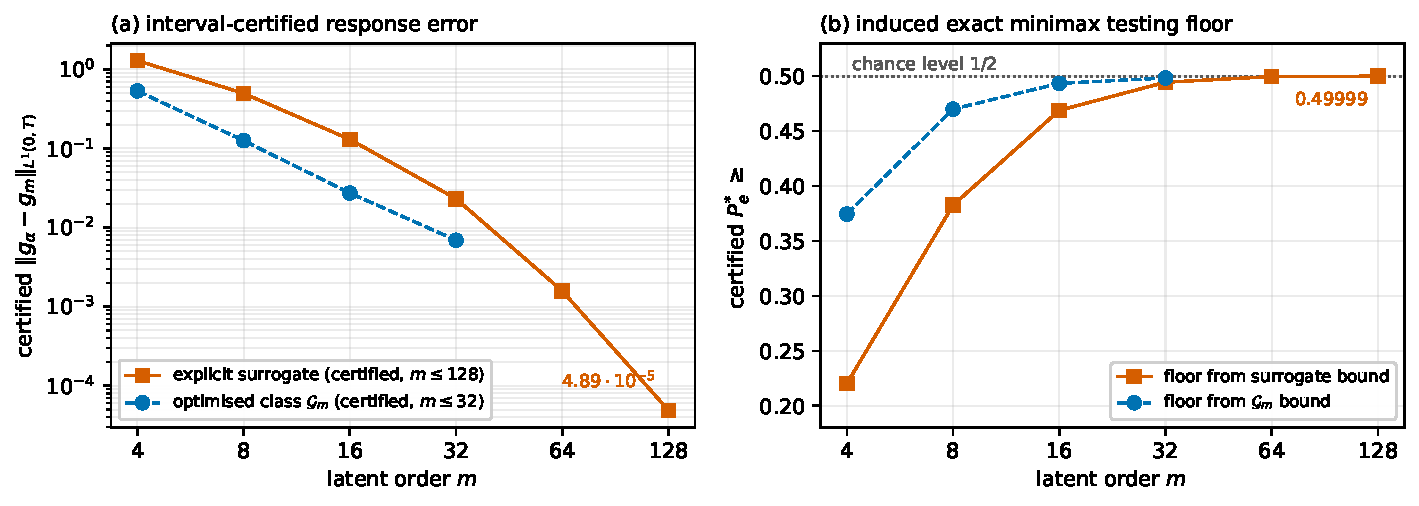
\includegraphics[width=0.98\textwidth]{fig_cert_floor.pdf}
\caption{The certified indistinguishability floor (Theorem~\ref{thm:floor} with Table~\ref{tab:cert}; certified content). (\textbf{a}) Interval-certified $L^{1}$ response errors: the optimized class $\mathcal{G}_{m}$ to $m=32$ and the explicit surrogate of Section~\ref{sec:reduction} to $m=128$; the latter is one admissible element, so it upper-bounds the class error. (\textbf{b}) The induced exact minimax floor: above $0.4996$ at $m=64$ and above $0.49998$ at $m=128$, uniformly over all inputs with $\|u\|_{2}\le0.120$. At attainable latent orders the finite-state rival cannot be distinguished from the fractional law under this protocol by any admissible experiment.}
\label{fig:certfloor}
\end{figure}

\begin{Remark}
The floor is one-sided: a value near $1/2$ proves that the declared protocol cannot separate $g_{\alpha}$ from at least one admitted rival; a small floor proves nothing in the converse direction. The certificate covers the linearized prey response at the stated cell; the nonlinear benchmark of Section~\ref{sec:numerics} corroborates the same obstruction at the trajectory level, where the pooled latent-class recall (Section~\ref{sec:numerics}) never exceeds $0.55$ for any classical design.
\end{Remark}

%=====================================================================
\section{Safe Discrimination Beyond Classical Waveforms}
\label{sec:safe}

The second principal finding is empirical, and it corrects a conclusion that the classical experiment designs invite. Throughout this section the decision layer is a four-class Bayesian-information-criterion (BIC) selection among the response laws of Section~\ref{sec:model}, evaluated on simulated trajectories with the declared noise; all accuracy statements are corroboration in the sense of Section~\ref{sec:intro}, while the safety statements carry the graded rigor of Section~\ref{sec:safety-status}.

\subsection{Six Classical Families and Their Frontier}

Six classical excitation families---pulse, sinusoid, multisine, multiscale, chirp, and a pseudorandom binary sequence (PRBS), Figure~\ref{fig:waveforms}---are compared at the common peak budget $\|u\|_{\infty}\le0.100$ on a stable-regime benchmark of $1512$ cells with $200$ noise replicates each (zero solver divergences). The frontier is stark: PRBS and multisine discriminate best (macro-accuracy $0.584$ and $0.583$) but cross the Allee threshold in $100\%$ and $35.7\%$ of stable cells, while the only family that never crosses (multiscale) scores $0.324$. Figure~\ref{fig:safetygeom} shows the geometry that produces the crossings.

\begin{figure}[H]
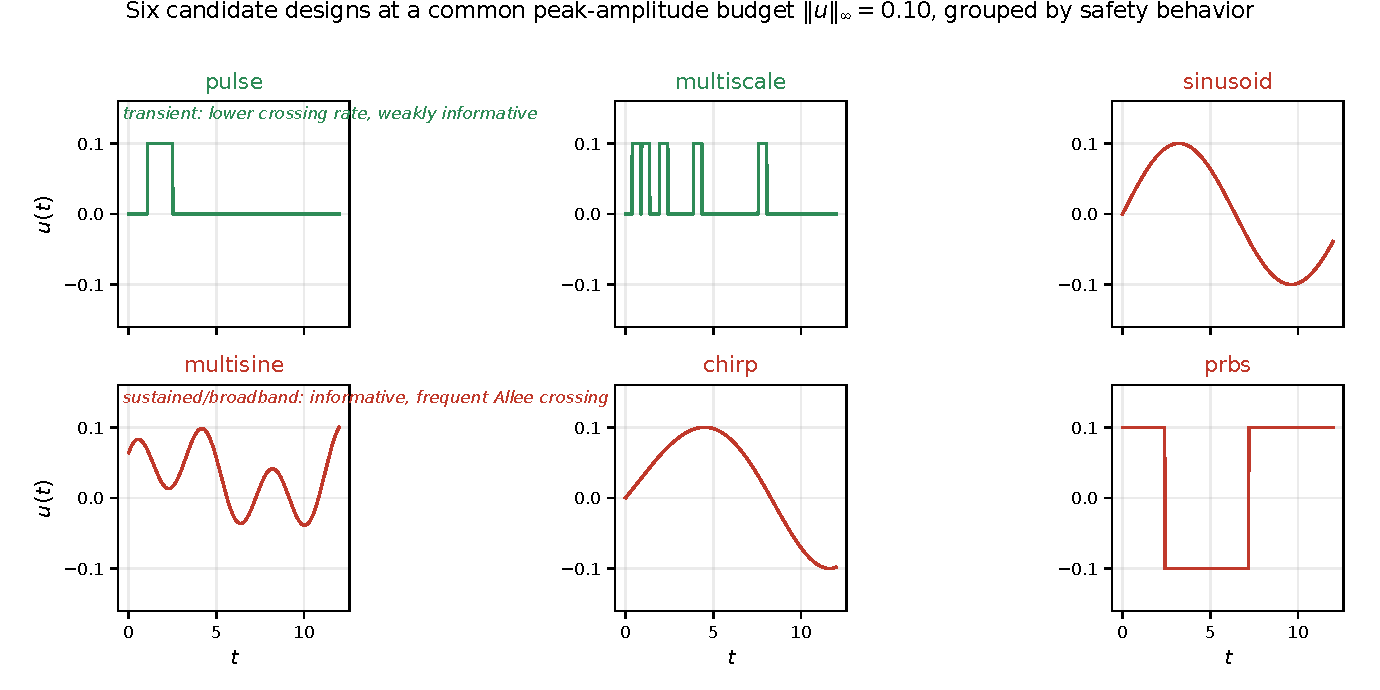
\includegraphics[width=0.85\textwidth]{fig04_waveforms.pdf}
\caption{The six classical excitation families at the common peak budget (exposition). Broadband and sustained inputs (PRBS, multisine, chirp, sinusoid) carry the discriminating energy but drive the prey toward the threshold; the transient families are gentle and uninformative. The searched designs of Section~\ref{sec:search} lie outside all six parameterizations.}
\label{fig:waveforms}
\end{figure}

\begin{figure}[H]
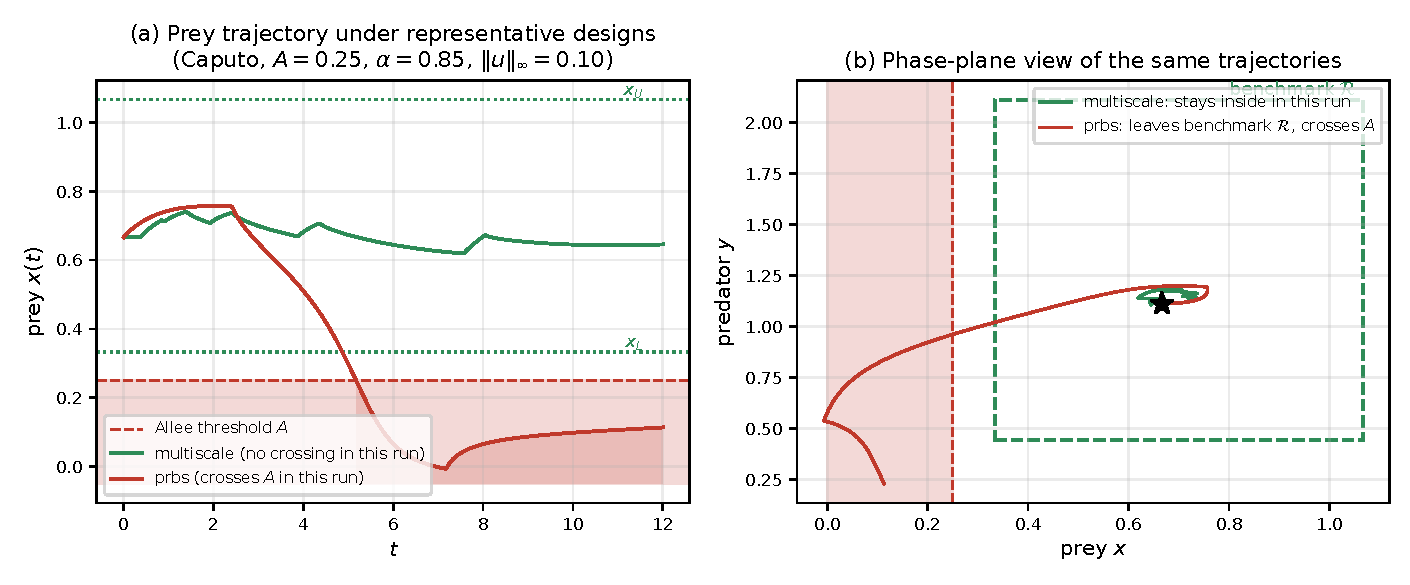
\includegraphics[width=0.62\textwidth]{fig15_safety_geometry.pdf}
\caption{Safety geometry (exposition): the coexistence equilibrium $x^{*}=2/3$, the Allee threshold $A$, and the margin $\min_{t}x(t)-A$ that every safety verdict in this paper measures. Crossing $A$ changes the basin structure and ends the identification experiment irreversibly; the dashed rectangle is a diagnostic region, not an invariant-set certificate.}
\label{fig:safetygeom}
\end{figure}

\subsection{Amplitude Is the Wrong Knob}
\label{sec:amplitude}

A natural reading of the frontier is that the excitation is simply too strong. Repeating the entire benchmark at peak amplitudes $0.050$ and $0.063$ alongside $0.100$ ($2268$ cells in total, zero divergences) refutes this: the design ordering is unchanged, PRBS remains the most informative input at every amplitude, and it still crosses in $71.4\%$ of cells at half amplitude ($92.9\%$ at $0.063$, $100\%$ at $0.100$). The realized response gain $\max_{t}|z(t)-z^{*}|/\|u\|_{\infty}$ explains why: for the crossing designs it \emph{increases} as the amplitude decreases, reaching $28.07$ at amplitude $0.050$ against the linear certificate $\Gamma_{T}=5.78$---a violation by a factor $4.86$---whereas the two never-crossing designs stay between $1.47$ and $2.06$, amplitude-independent, as a linear response must. Once a trajectory escapes the Allee basin, its excursion is set by the basin geometry rather than by the input, so the ratio scales like $1/\|u\|_{\infty}$. Shrinking the input does not convert an unsafe design into a safe one, and the linear certificate cannot license safety for any crossing design at any tested amplitude.

\subsection{The Waveform Search}
\label{sec:search}

If amplitude is not the knob, the waveform shape may be. We searched for inputs that are safe \emph{and} informative outside the six families, at the same peak budget and under the hard constraint that the minimum Allee margin over all four candidate laws be at least $\delta=0.05$. The search covers piecewise-constant inputs with $4$, $6$, and $8$ levels, free multisines with $3$--$6$ harmonics, and pulse trains with $2$--$4$ pulses, scored by the minimax pairwise separation $J(u)=\min_{a\neq b}\|\mu_{a}(u)-\mu_{b}(u)\|/\sigma$ over the four classes; $163{,}840$ candidates were evaluated by scrambled Sobol sampling (fixed seed) with Nelder--Mead refinement of the per-family best, and $87{,}601$ ($53.5\%$) satisfy the safety constraint. Under the identical objective, exactly one classical design is safe at this budget (multiscale, $J=1.45$)---and it is the least informative of the six---while the best safe candidate found reaches $J=6.23$, and every one of the twelve best safe candidates is piecewise constant, a class the six families do not contain.

Validating the six leading candidates with the same BIC classifier, the same $56$-cell grid, and the same replicate seeds as the benchmark confirms the surrogate objective. All six are safe, with zero observed crossings and verified margins between $+0.067$ and $+0.176$, and five of the six outrank the best classical design of \emph{any} kind. The leading design---a six-level piecewise-constant input with levels $(+0.513,-0.735,+0.692,+0.469,-0.712,-0.353)$ in units of the peak budget on equal subintervals of $[0,T]$---attains macro-accuracy $0.803$, against $0.514$ for the only safe classical design and $0.763$ for multisine, which crosses in $35.7\%$ of cells. The gain concentrates exactly where the safe classical design fails: Caputo recall rises from $0.404$ to $0.911$ and delay recall from $0.445$ to $0.853$. Figure~\ref{fig:frontier} displays the resulting design plane.

\begin{figure}[H]
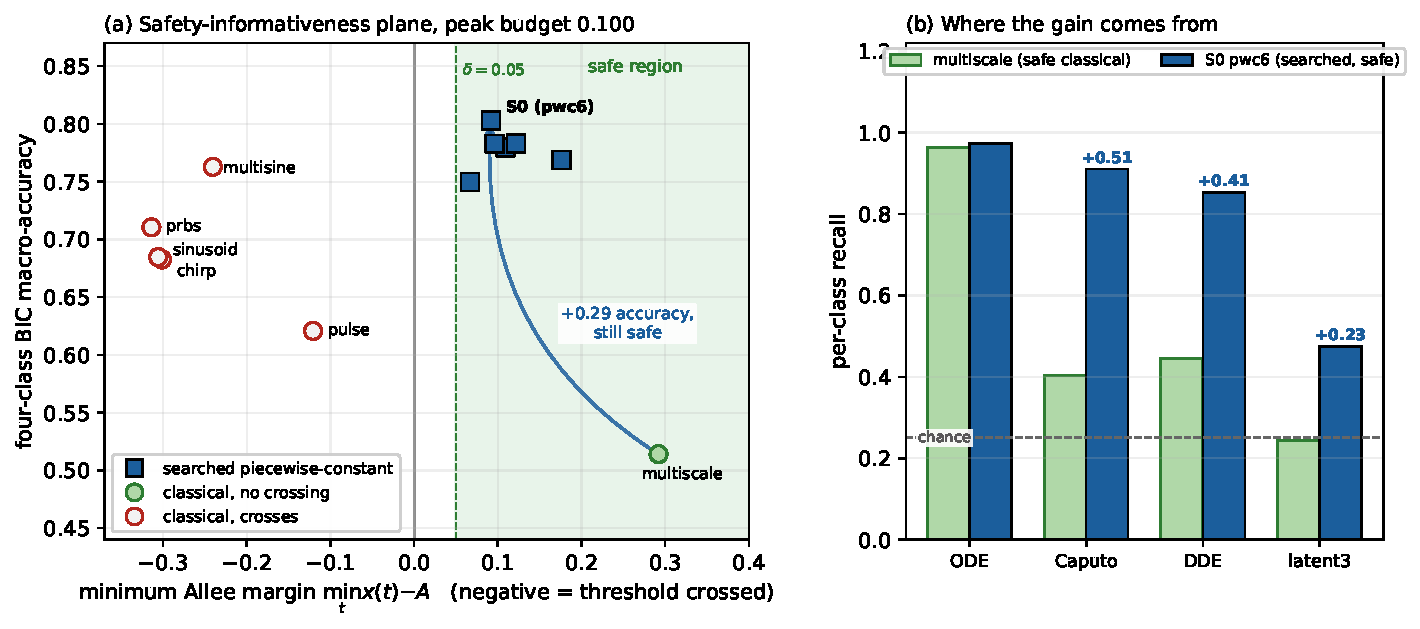
\includegraphics[width=0.98\textwidth]{fig24_safe_design_frontier.pdf}
\caption{The safety--informativeness plane at the common peak budget (corroboration; safety status per Section~\ref{sec:safety-status}). (\textbf{a}) Minimum Allee margin over the four candidate laws against four-class BIC macro-accuracy ($56$ cells $\times$ $100$ replicates, identical seeds): circles are the six classical families (filled when no crossing occurs), squares the leading searched designs. Of the twelve designs, only multiscale and the searched six-level piecewise-constant input are safe under \emph{all four} laws, and the searched designs occupy a region the classical families do not reach. (\textbf{b}) Per-class recall of the safe classical design against the leading searched design; the gain concentrates on the Caputo and delayed mechanisms. The search establishes \emph{existence}---Sobol sampling with local refinement, one amplitude, one $\alpha$---not a certified global optimum.}
\label{fig:frontier}
\end{figure}

\begin{table}[H]
\caption{Validation of the leading searched designs against the six classical families with the benchmark classifier ($56$ cells $\times$ $100$ replicates per design, identical seeds, no divergences; corroboration). \textsc{pwc}$k$: $k$-level piecewise-constant input on equal subintervals; S0--S5: the six leading searched candidates. The latent column pools generators of orders $1$ and $3$ (Proposition~\ref{prop:scope}(v)). Margins are the minimum over the four candidate laws; their rigor is graded in Section~\ref{sec:safety-status}.}
\label{tab:designs}
\begin{tabular}{lcccccc}
\toprule
design & family & macro & crossings & margin & Caputo rec. & delay rec.\\
\midrule
S0 & \textsc{pwc}6 & \textbf{0.803} & 0.000 & $+0.092$ & 0.911 & 0.853\\
S3 & \textsc{pwc}6 & 0.783 & 0.000 & $+0.122$ & 0.910 & 0.927\\
S2 & \textsc{pwc}6 & 0.783 & 0.000 & $+0.096$ & 0.875 & 0.816\\
S1 & \textsc{pwc}6 & 0.780 & 0.000 & $+0.109$ & 0.838 & 0.897\\
S5 & \textsc{pwc}8 & 0.769 & 0.000 & $+0.176$ & 0.844 & 0.926\\
multisine & classical & 0.763 & 0.357 & $-0.240$ & 0.844 & 0.902\\
S4 & \textsc{pwc}6 & 0.750 & 0.000 & $+0.067$ & 0.766 & 0.743\\
PRBS & classical & 0.711 & 1.000 & $-0.314$ & 0.802 & 0.521\\
sinusoid & classical & 0.685 & 1.000 & $-0.306$ & 0.844 & 0.549\\
chirp & classical & 0.683 & 0.929 & $-0.301$ & 0.832 & 0.547\\
pulse & classical & 0.621 & 0.071 & $-0.121$ & 0.528 & 0.647\\
multiscale & classical & 0.514 & 0.000 & $+0.292$ & 0.404 & 0.445\\
\bottomrule
\end{tabular}
\end{table}

Two readings of Table~\ref{tab:designs} matter. Every searched design is safe with margin at least $+0.067$, five of six outrank the best classical design of any kind, and the two designs safe under \emph{all four} laws---multiscale and S0---differ by $0.289$ in macro-accuracy. And the constraint is active: the leading designs sit near the declared margin $\delta=0.05$ while multiscale sits at $0.292$, so the Pareto trade is relocated, not abolished (Proposition~\ref{prop:scope}(ii)).

A design selected and evaluated at one operating point could be overfitted to it. The validation grid answers this without extra computation: the search ran at $A=0.25$ only, while the grid also contains $A=0.20$, which is fully held out. On the held-out threshold the searched designs lose on average $0.060$ macro-accuracy while the six classical families---never optimized at all---lose $0.087$; the best searched design still leads the best classical design out of sample ($0.907$ against $0.837$), and its advantage over the safe classical design is \emph{larger} out of sample ($+0.486$) than in sample ($+0.255$). There is no evidence that the advantage is an in-sample artifact.

\subsection{Safety Status of the Headline Trajectories}
\label{sec:safety-status}

Safety verdicts carry three grades of rigor, stated exactly. \emph{First}, every reported trajectory is verified a posteriori: the solver output is refined until the minimum prey value stabilizes, and the gap between mesh nodes is closed by a rigorous modulus-of-continuity bound from the Caputo mild solution, so no crossing can hide between samples; across the $28$ trajectories tested ($7$ designs $\times$ $4$ laws) every verdict is decided, $12$ safe and $16$ crossing, and each agrees with the benchmark's sampled classification. \emph{Second}, for the two headline designs under the integer-order and finite-latent laws---four trajectories---a validated enclosure holds: a piecewise-cubic reference with an interval-bounded defect (convergence order $2.0$, defect $5.9\cdot10^{-9}$ at the finest mesh) and a one-sided log-norm Gr\"onwall estimate give self-consistent error bounds of $4.6\cdot10^{-3}$ and $4.2\cdot10^{-2}$, hence rigorous lower bounds $0.441$ and $0.309$ on the prey minimum against $A=0.25$. Only these four are called rigorous. \emph{Third}, the delayed and Caputo trajectories are verified but not enclosed: the delayed defect stalls at first order because input discontinuities re-enter through the retarded argument, and the fractional defect is limited by the solver's own order; both failure modes are structural and are stated rather than hidden.

Two further facts calibrate what an invariant-set alternative could deliver. The quadratic-remainder constant of the field \eqref{eq:field} admits the interval-certified bound $M_{2}(r)\le5.47$ at radius $r=0.05$ (sampling underestimates it by $19\%$), giving a certified invariant-ball radius $r_{\max}=0.0294$---twelve times smaller than the ecological margin it must protect---and a certified admissible amplitude $U_{\mathrm{NL}}=1.42\cdot10^{-3}$, seventy times below the budget actually used. The invariant-ball route to nonlinear safety is therefore closed for this field, and a posteriori verification is the operative tool.

\subsection{Scope}

\begin{Proposition}[what is and is not established]
\label{prop:scope}
(i) Theorem~\ref{thm:floor} with Table~\ref{tab:cert} is a certified statement about the linearized prey response at $(\alpha,A)=(0.85,0.25)$, $T=12$, uniform over inputs with $\|u\|_{2}\le0.120$ and over sampling schedules; it does not classify the nonlinear trajectories. (ii) The search of Section~\ref{sec:search} establishes existence of safe designs above the classical frontier at one amplitude and one $\alpha$; no certified global optimum over any waveform class is claimed, and the safety constraint is active at the declared margin $\delta=0.05$, so a stricter margin buys a lower objective: a Pareto cost remains and safety is not free. (iii) Local stability facts are inherited from \cite{Companion} and nothing here implies global asymptotic stability, basin geometry, or bifurcation classification. (iv) Accuracy numbers are corroboration under the declared BIC protocol; changing the decision rule changes them, and the floor of Section~\ref{sec:floor} is the only decision-rule-independent statement. (v) The benchmark's latent class pools data generated at latent orders $m=1$ and $m=3$ against the single $m=3$ hypothesis; class-wise statistics are pooled accordingly. (vi) The case study of Section~\ref{sec:case} is empirically \emph{anchored}, not calibrated: its growth coefficient, Allee threshold, and memory mechanisms are declared scenario choices, and its conclusions are structural, not quantitative ecology.
\end{Proposition}

%=====================================================================
\section{Numerical Corroboration and Validation}
\label{sec:numerics}

All computations in this section are corroboration; their role is to stress-test the theorems and the search result, not to prove them.

\subsection{Solver Self-Tests and Reproducibility Controls}

Caputo trajectories use the fractional Adams--Bashforth--Moulton predictor--corrector scheme of \cite{Diethelm2002}; the integer-order and delay laws use classical fourth-order Runge--Kutta with interpolated history. The scalar self-test against the exact Mittag-Leffler solution $E_{\alpha}(\lambda t^{\alpha})$ gives maximum errors $8.7\cdot10^{-4}$, $4.6\cdot10^{-4}$, $2.5\cdot10^{-4}$ at $N=250,500,1000$ steps (Figure~\ref{fig:solver}), the expected first-order-plus-$\alpha$ trend at production resolution. Because the four candidate laws are integrated on the same grid inside the BIC comparison, a common discretization bias largely cancels in the decision statistic. As a cross-host control, the frozen benchmark was re-run on an independent machine under a re-implemented driver and different library versions: macro-accuracy and the per-design accuracies and crossing rates reproduce to four decimal places ($0.5369$ vs.\ $0.537$; $0.5836$ vs.\ $0.584$; $0.5829$ vs.\ $0.583$; $0.3235$ vs.\ $0.324$), with identical crossing rates.

\begin{figure}[H]
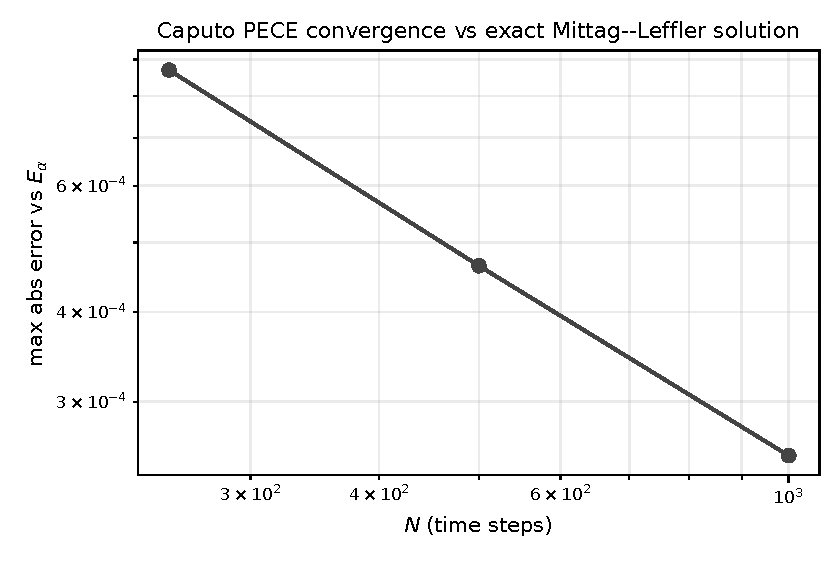
\includegraphics[width=0.55\textwidth]{fig06_solver_convergence.pdf}
\caption{Solver self-test (corroboration): maximum error of the predictor--corrector scheme against the exact Mittag-Leffler solution under mesh refinement. The benchmark's production resolution sits at the right end; the trend, not any single value, is the control.}
\label{fig:solver}
\end{figure}

\subsection{The Four-Class Benchmark}

Figure~\ref{fig:benchmark} summarizes the stable-regime task. The dominant failure mode is conservative collapse toward the simplest explanation: the integer-order class has recall $0.972$ but precision $0.227$ under weak excitation, a Caputo verdict is nearly always correct once issued (precision $0.984$), and the pooled latent class (generators of orders $m\in\{1,3\}$ scored against the single $m=3$ hypothesis; Proposition~\ref{prop:scope}(v)) has recall $0.242$---consistent with the certified floor of Section~\ref{sec:floor}, though the BIC dimension penalty acts in the same direction and the two effects are not separated here, so the benchmark recall is not offered as evidence for the floor. Accuracy falls toward the integer limit ($0.702$ at $\alpha=0.70$ to $0.312$ at $\alpha=0.95$) and rises with the signal-to-noise ratio; observing both species is best, and the directly actuated prey channel remains structurally sufficient.

\begin{figure}[H]
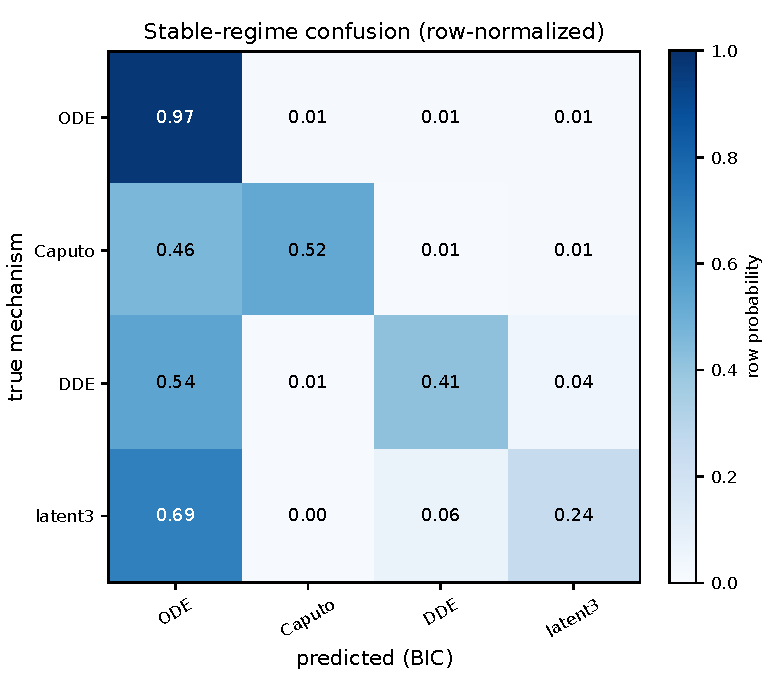
\includegraphics[width=0.48\textwidth]{fig07_confusion.pdf}
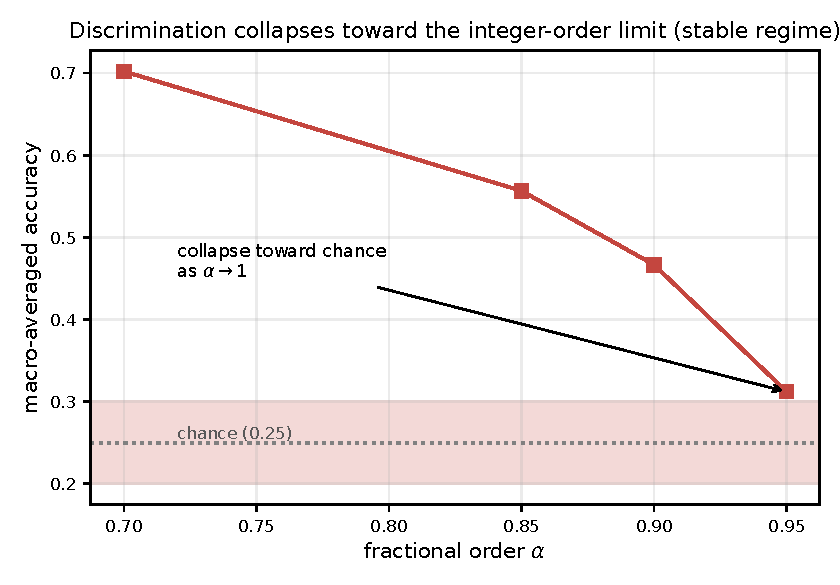
\includegraphics[width=0.48\textwidth]{fig08_accuracy_vs_alpha.pdf}
\caption{The four-class benchmark (corroboration; $1512$ cells $\times$ $200$ replicates, no divergences). Left: row-normalized confusion; the latent row pools generators of orders $1$ and $3$ against the $m=3$ hypothesis. Right: accuracy against the fractional order; discrimination degrades as $\alpha\to1$, where the mechanisms coincide. Both panels condition the reading of the search result: the searched designs of Figure~\ref{fig:frontier} move the whole frontier, they do not remove the $\alpha\to1$ degeneracy or the latent obstruction.}
\label{fig:benchmark}
\end{figure}

\subsection{The Protocol-Restricted Atlas and the Fractional-Delay Bridge}

Two further layers place the results in parameter space. First, applying the floor of Theorem~\ref{thm:floor} across $(\alpha,A,m)$ yields a protocol-restricted discrimination atlas (Figure~\ref{fig:atlas}): the testing bound rises toward chance with $m$ everywhere, and cells violating the Matignon stability condition $\alpha<\alpha^{*}(A)$ of \cite{Companion} are excluded from stable-regime conclusions. Second, a combined fractional-delay law---equal to the Caputo system at $\tau=0$ and to the delay system at $\alpha=1$---was simulated over $(\alpha,\tau)\in[0.70,1]\times[0,0.5]$; interior cells occupy response regions far from both limits (distance $0.28$ to the Caputo limit and $0.69$ to the delay limit at $(\alpha,\tau)=(0.95,0.50)$; Figure~\ref{fig:bridge}), so fitting the two endpoint models separately cannot reveal a composite mechanism, and designs should test composite alternatives rather than endpoints only.

\begin{figure}[H]
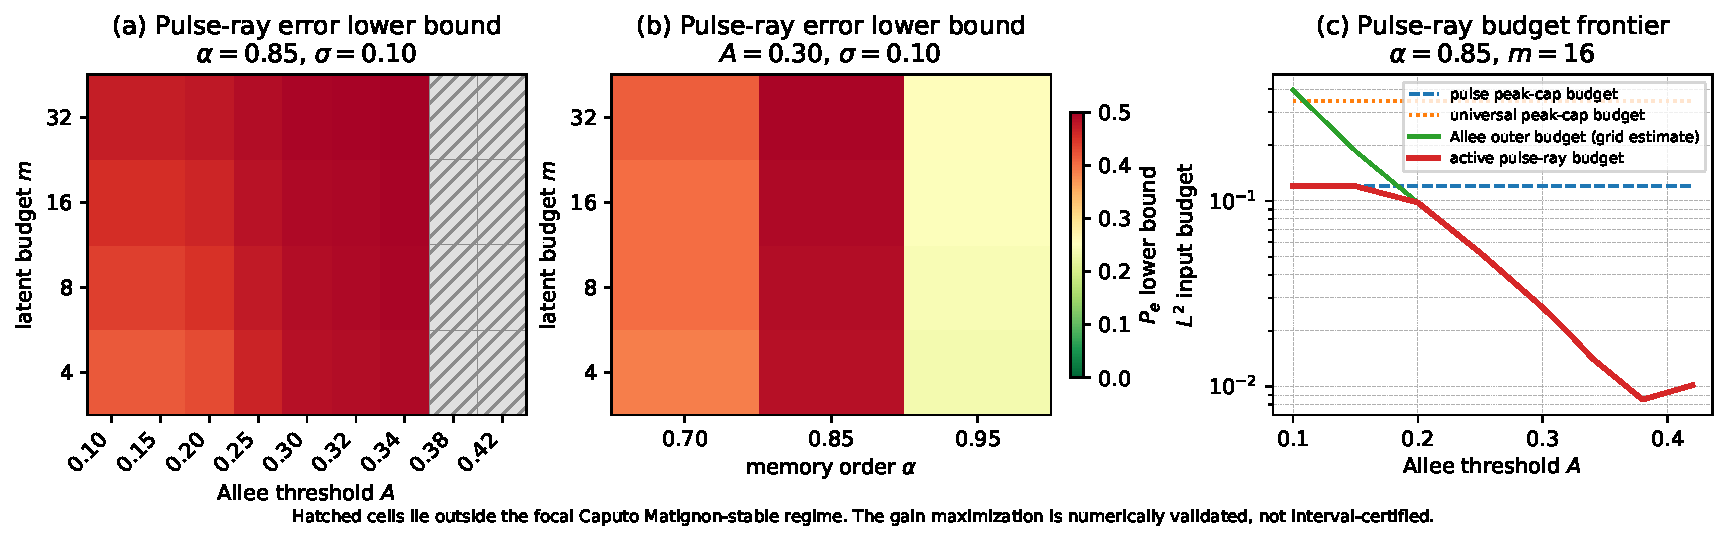
\includegraphics[width=0.6\textwidth]{fig18_safe_discrimination_atlas.pdf}
\caption{Protocol-restricted discrimination atlas over $(\alpha,A,m)$ (certified floor applied cell-wise): lower bound on the model-selection error under the declared pulse protocol. Hatched cells violate the Matignon condition $\alpha<\alpha^{*}(A)$ and are excluded. The floor increases with the latent budget $m$ in every admissible cell.}
\label{fig:atlas}
\end{figure}

\begin{figure}[H]
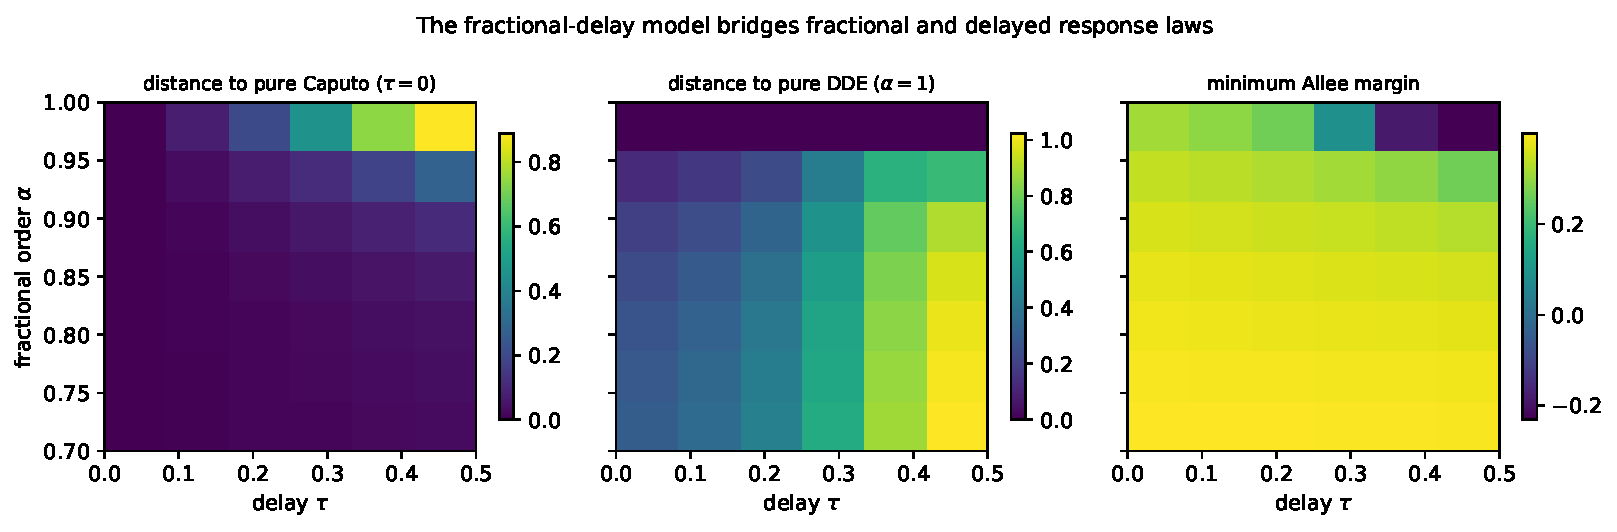
\includegraphics[width=0.62\textwidth]{fig21_fractional_delay_bridge.pdf}
\caption{The fractional-delay bridge (corroboration): responses of the combined law at interior $(\alpha,\tau)$ against the pure-Caputo and pure-delay limits. Interior cells sit far from both endpoints simultaneously, so endpoint fitting cannot detect a composite mechanism; this motivates including composite alternatives in the candidate set of a real experiment.}
\label{fig:bridge}
\end{figure}

%=====================================================================
\section{An Empirically Anchored Case Study: the Boreal Vole--Weasel System}
\label{sec:case}

The benchmark parameters are exact rationals chosen for arithmetic convenience. To test whether the paper's statements survive contact with an empirically grounded parameterization, we instantiate the model \eqref{eq:field} on the boreal vole--weasel interaction, the classical specialist-predator system of Fennoscandian population ecology, and re-run every layer of the analysis---exact invariants, certified floor, trajectory safety, and the four-class discrimination task---at that point. All computations in this section reuse the machinery of Sections~\ref{sec:floor} and~\ref{sec:safe} unchanged; only the parameters differ.

\subsection{Parameterization and Its Declared Limits}

Prey carrying capacity, the specialist functional response, and predator demography are anchored to the Turchin--Hanski vole--weasel parameterization \cite{TurchinHanski1997}: $K=150$ voles\,ha$^{-1}$, a Holling type-II response with maximum consumption $Q=600$ voles\,yr$^{-1}$\,weasel$^{-1}$ and half-saturation $D_{0}=6$ voles\,ha$^{-1}$ (hence $a=Q/D_{0}=100$, $h=1/D_{0}=1/6$ in the notation of \eqref{eq:field}), and weasel loss rate $\mu=1.25$\,yr$^{-1}$. Three mapping decisions are scenario choices, stated as such. First, the net prey growth coefficient $r=1.0$\,yr$^{-1}$ absorbs the generalist-predation term that \cite{TurchinHanski1997} model separately. Second, a strong Allee threshold is not empirically documented for \emph{Microtus}; we impose $A=37.5$ voles\,ha$^{-1}$ as a scenario replicating the benchmark's relative geometry ($A/K=1/4$, $x^{*}/K=2/3$), in the spirit of demographic Allee mechanisms reviewed in \cite{Courchamp2008}. Third, the weasel efficiency $e=53/24000$ places the coexistence equilibrium at $x^{*}=100$ voles\,ha$^{-1}$, giving $y^{*}=53/540\approx0.098$ weasels\,ha$^{-1}$---about ten per square kilometre---and the fractional, delayed, and latent response laws are competing scenario mechanisms, exactly as in the benchmark. No claim of calibration is made; the case study asks whether the \emph{structure} of the results persists at an empirically sensible operating point.

\subsection{The Cell Is a Fractional-Stabilization Regime}

All equilibrium invariants are exact rationals: $\operatorname{tr}J=16/53$, $\det J=25/636$, with complex eigenvalues and critical order $\alpha^{*}(A)=0.4491$. The integer-order equilibrium is therefore \emph{unstable}, while the Caputo law at the scenario order $\alpha=0.40<\alpha^{*}$ is Matignon-stable: the case study operates in the fractional-stabilization regime whose atlas is certified in the companion study \cite{Companion}. Two structural consequences follow immediately and are visible in every experiment below. Because only the fractional law is locally stable, safety verdicts depend on the \emph{true} mechanism far more strongly than at the benchmark cell, which vindicates the all-four-laws worst-case safety criterion of Section~\ref{sec:model}. And because the functional response is nearly saturated at the equilibrium ($x^{*}/(D_{0}+x^{*})=0.943$), the delayed trophic pathway is almost unobservable: perturbing $x(t-\tau)$ barely moves the predation term, so the delayed law is empirically indistinguishable from the integer one at this operating point---a concrete, falsifiable prediction of the analysis.

\subsection{The Certified Floor Persists}

Re-running the certification of Section~\ref{sec:reduction} at the case cell---partial-fraction poles $\rho_{1,2}=(96\pm2i\sqrt{1671})/25$, now with \emph{positive} real part, $|\mu|=\sqrt{25/636}<1/5$, $\alpha=2/5$---yields interval-certified response errors $\|g_{\alpha}-g_{m}\|_{L^{1}}\le 1.2609$, $0.2151$, $0.04535$, $5.821\cdot10^{-3}$, $1.809\cdot10^{-4}$, $3.141\cdot10^{-6}$ at $m=4,\dots,128$, with certified floors $0.2247$, $0.4487$, $0.4891$, $0.4986$, $0.49996$, and $0.4999992$. All surrogate poles are again certified by interval Newton, and every one of them has negative real part at every order: the positive exponential-sum surrogate inherits stability even in the fractional-stabilization regime, in sharp contrast to the memoryless discretizations of \cite{Companion}. The indistinguishability obstruction is thus not an artifact of the benchmark rationals; at the empirically anchored cell it is, if anything, slightly stronger.

\subsection{Safety Inverts; the Searched Design Transfers}

Figure~\ref{fig:casetraj} shows the four laws under two designs at the relative amplitude $8\%\,x^{*}$ ($8$ voles\,ha$^{-1}$\,yr$^{-1}$). The safety geometry \emph{inverts} relative to the benchmark: multiscale---the only safe classical family there---now drives every non-fractional law across the Allee threshold to extinction (margins $-38$ to $-39$ voles\,ha$^{-1}$), because its slow forcing resonates with the unstable spiral of the integer dynamics, while the fractional law remains safely stabilized ($+19.3$). Broadband PRBS, lethal at the benchmark, is here the most conservative classical input ($+54.9$). Safety rankings are regime-dependent, and only the worst-case criterion over candidate laws survives the change of operating point. The searched design S0, transferred verbatim from the benchmark with no re-optimization, is safe under all four laws (worst margin $+16.5$).

\begin{figure}[H]
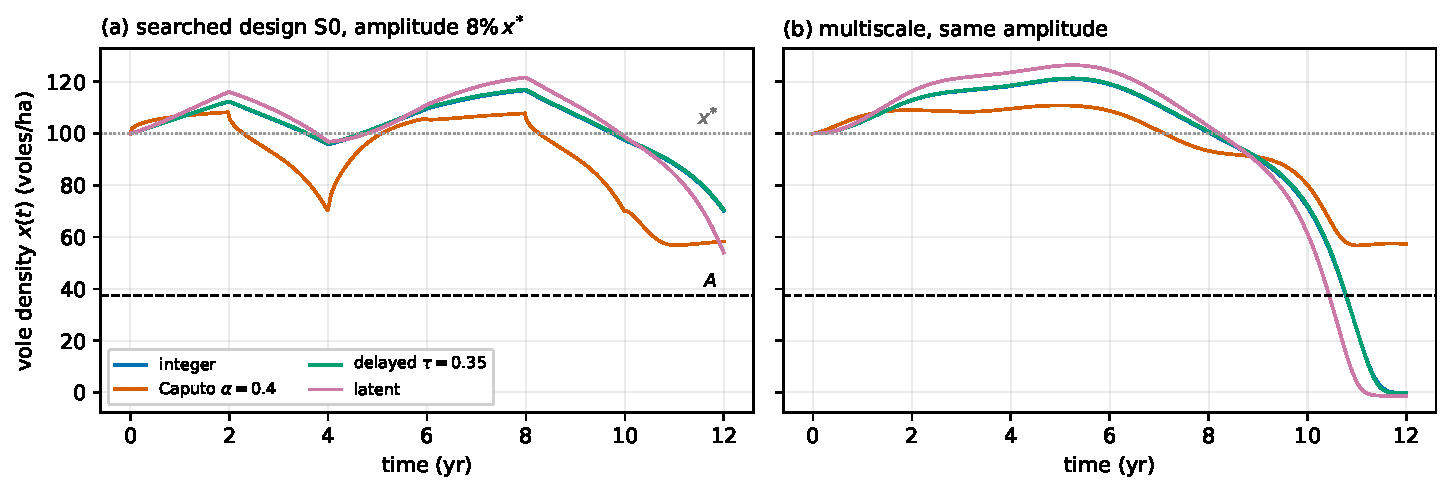
\includegraphics[width=0.98\textwidth]{fig_case_traj.pdf}
\caption{Case-study trajectories at amplitude $8\%\,x^{*}$ (corroboration; threshold $A=37.5$ dashed, equilibrium $x^{*}=100$ dotted). (\textbf{a}) The searched design S0 keeps all four laws above the threshold (worst margin $+16.5$ voles\,ha$^{-1}$, under the latent law). (\textbf{b}) Multiscale forcing drives the integer, delayed, and latent laws across $A$ to collapse near year~$10.5$, while the Caputo law at $\alpha=0.40<\alpha^{*}=0.449$ is fractionally stabilized; the integer curve is hidden beneath the delayed one, illustrating the near-unobservability of the delay at this saturated operating point.}
\label{fig:casetraj}
\end{figure}

\subsection{The Discrimination Plane at the Case Cell}

Figure~\ref{fig:casedesign} reports the four-class BIC task ($100$ replicates per cell, two SNR levels, prey and both-species channels, deterministic seeds). The structure of Section~\ref{sec:search} recurs: the accuracy-leading design (multiscale, macro $0.627$) is the one that destroys the system under three of the four candidate laws, and among designs safe under all four laws the transferred S0 leads (macro $0.574$), ahead of every safe classical input by at least $0.12$. The delayed class is never recovered (recall $\le0.01$ for every design)---the saturation prediction above, realized in the decision layer---so the case-study task is effectively three-class, and macro-accuracy is depressed accordingly for all designs. As at the benchmark, the latent class is hardest among the observable ones, consistent with the certified floor.

\begin{figure}[H]
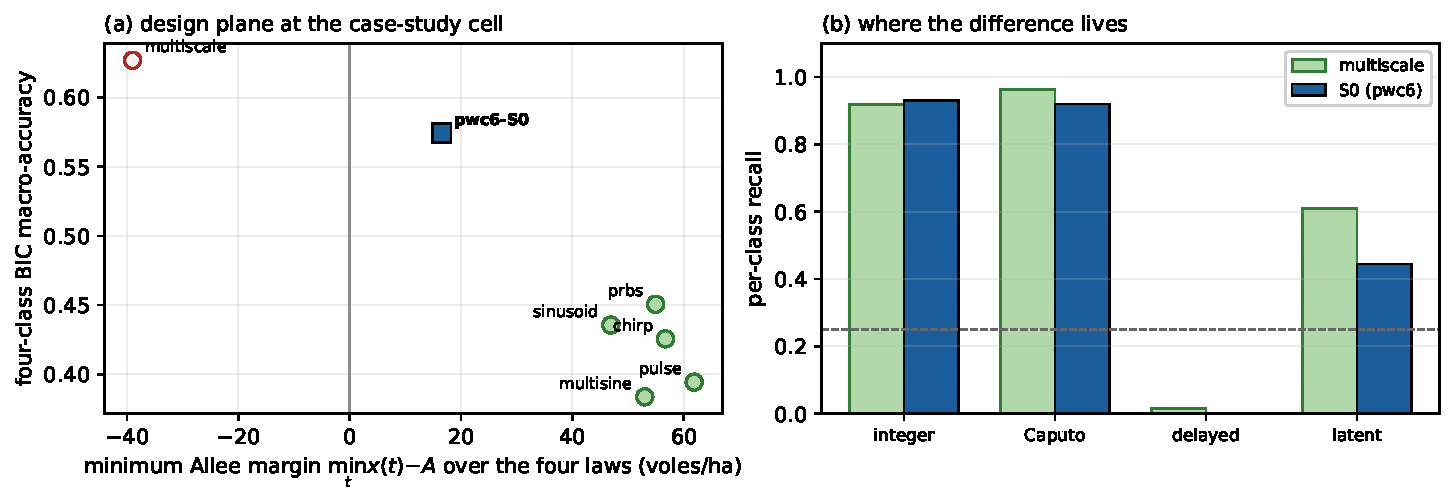
\includegraphics[width=0.98\textwidth]{fig_case_design.pdf}
\caption{The case-study design plane (corroboration). (\textbf{a}) Minimum Allee margin over the four laws against four-class BIC macro-accuracy: multiscale buys its accuracy lead by crossing the threshold ($-39$ voles\,ha$^{-1}$); among all-law-safe designs the benchmark-searched S0 leads without re-optimization. (\textbf{b}) Per-class recall for the two leading designs: the delayed law is unrecoverable at this operating point (functional-response saturation), and the latent law remains the hardest observable class.}
\label{fig:casedesign}
\end{figure}

In summary, the paper's three principal statements---the certified floor, the artifactual character of the classical safety--informativeness frontier, and the necessity of a worst-case safety criterion over candidate mechanisms---all persist at the empirically anchored cell, and the case study adds one prediction of independent ecological interest: at saturated specialist-predation operating points, gestation-delay mechanisms are practically unidentifiable from perturbation data.

%=====================================================================
\section{Discussion and Conclusions}
\label{sec:discussion}

\subsection{What Is New, and What Is for Completeness}

The certified indistinguishability floor (Theorem~\ref{thm:floor} with Table~\ref{tab:cert}) and the scalar reduction that makes its $m=128$ certification possible (Section~\ref{sec:reduction}) are the analytic and certified core. The endpoint-inclusive Lemma~\ref{lem:soe} is a supporting tool whose technique belongs to the cited literature. The refutation of the classical safety--informativeness frontier is the principal empirical finding, with its safety layer graded as in Section~\ref{sec:safety-status}. The structural separation (Theorem~\ref{thm:sep}), the solver validation, and the benchmark machinery are completeness.

\subsection{The Two-Sided Conclusion}

The two principal results point in opposite directions, and their combination is the message. Downward: no waveform, of any shape, within the declared budget, can distinguish the fractional response from a latent surrogate of order $128$---the certified floor is $0.49998$ against the chance level $0.5$, uniformly over inputs. Upward: within the same budget, the apparent conflict between safety and informativeness dissolves under waveform search---a safe piecewise-constant design recovers $0.803$ of the four-class task, against $0.514$ for the best safe classical family, with the advantage persisting out of sample. The operative constraint on identifying ecological memory is therefore the declared rival-complexity budget $m$, together with the proximity of $\alpha$ to $1$, and not the safety margin; the vole--weasel case study shows that this reading, and the worst-case safety criterion it relies on, survive transport to an empirically anchored operating point where the safety ranking of individual designs is inverted. For experimental practice the consequence is a change of question: not \emph{which model fits best}, nor \emph{which safe perturbation separates the mechanisms}---that now has a constructive answer---but \emph{what latent complexity the experiment is willing to admit as a rival}. The allowed latent dimension, delay range, forcing bandwidth, and observation horizon belong in the scientific specification of an experiment alongside organism and protocol, because that declaration, not the safety margin, bounds what can be identified.

\subsection{Which Conclusions Admit an Ecological Reading, and Which Do Not}

The locked parameters are exact rationals chosen for arithmetic convenience and are not calibrated to any organism; no numerical value here carries empirical meaning. What does admit a structural reading is the mechanism content: informative excitation fails through basin escape, whose signature is a realized gain scaling like the reciprocal amplitude (Section~\ref{sec:amplitude}); and safe informative excitation exists but is not found inside textbook waveform families.

\subsection{Evidence Boundaries and Open Problems}

Every claim in the abstract traces to a theorem, a certified table, a named experiment, or a citation, with scope fixed by Proposition~\ref{prop:scope}. Open problems: (i) whether the boundary rate $c=\pi\sqrt{\alpha(1-\alpha)}$ in Lemma~\ref{lem:soe} is attained or optimal; (ii) a certified global optimum over the piecewise-constant class, upgrading the existence result of Section~\ref{sec:search}; (iii) validated enclosures for the delayed and Caputo headline trajectories, whose structural obstacles are identified in Section~\ref{sec:safety-status}; (iv) a decision layer without a dimension penalty, separating the certified floor from the BIC preference for small models; and (v) the analogous program for spatially extended or noisy-dynamics versions of the model, where the notion of a safe margin itself requires care.

\subsection{Conclusions}

For a locked strong-Allee ecology under Caputo, delayed, integer, and finite-latent response laws, we have combined an exact two-point minimax bound with interval-certified surrogate errors---made possible at latent order $128$ by a partial-fraction reduction and interval-Newton pole certification---into an indistinguishability floor that no admissible experiment can beat, and we have shown empirically that the safety--informativeness frontier suggested by classical waveform families is an artifact of the parameterization, refuted by explicitly constructed safe designs whose advantage survives a held-out control. Identification of ecological memory is budget-limited, not safety-limited.

\vspace{6pt}

\authorcontributions{The author performed the conceptualization, methodology, formal analysis, software, investigation, validation, data curation, visualization, and writing of this work. The author has read and agreed to the published version of the manuscript.}

\funding{This research received no external funding.}

\conflictsofinterest{The author declares no conflicts of interest.}

\reftitle{References}

\begin{thebibliography}{999}

\bibitem{Podlubny1999} Podlubny, I. \textit{Fractional Differential Equations}; Mathematics in Science and Engineering 198; Academic Press: San Diego, CA, USA, 1999.

\bibitem{Diethelm2010} Diethelm, K. \textit{The Analysis of Fractional Differential Equations}; Lecture Notes in Mathematics 2004; Springer: Berlin/Heidelberg, Germany, 2010.

\bibitem{Kilbas2006} Kilbas, A.A.; Srivastava, H.M.; Trujillo, J.J. \textit{Theory and Applications of Fractional Differential Equations}; North-Holland Mathematics Studies 204; Elsevier: Amsterdam, The Netherlands, 2006.

\bibitem{Mainardi2010} Mainardi, F. \textit{Fractional Calculus and Waves in Linear Viscoelasticity}; Imperial College Press: London, UK, 2010.

\bibitem{Ahmed2007} Ahmed, E.; El-Sayed, A.M.A.; El-Saka, H.A.A. Equilibrium points, stability and numerical solutions of fractional-order predator--prey and rabies models. \textit{J. Math. Anal. Appl.} \textbf{2007}, \emph{325}, 542--553.

\bibitem{Javidi2013} Javidi, M.; Nyamoradi, N. Dynamic analysis of a fractional order prey--predator interaction with harvesting. \textit{Appl. Math. Model.} \textbf{2013}, \emph{37}, 8946--8956.

\bibitem{Vargas2015} Vargas-De-Le\'on, C. Volterra-type Lyapunov functions for fractional-order epidemic systems. \textit{Commun. Nonlinear Sci. Numer. Simul.} \textbf{2015}, \emph{24}, 75--85.

\bibitem{Rihan2021} Rihan, F.A. Fractional-order delay differential equations with predator--prey systems. In \textit{Delay Differential Equations and Applications to Biology}; Forum for Interdisciplinary Mathematics; Springer: Singapore, 2021; pp.~211--232.

\bibitem{Companion} Alraddadi, I.; Alharthi, T.N. Exact stability atlases and a memoryless-surrogate failure theorem for a Caputo Allee predator--prey model. \textit{Mathematics} \textbf{2026}, in press.

\bibitem{Matignon1996} Matignon, D. Stability results for fractional differential equations with applications to control processing. In Proceedings of the Computational Engineering in Systems Applications, Lille, France, 9--12 July 1996; Volume 2, pp.~963--968.

\bibitem{Petras2011} Petr\'a\v{s}, I. \textit{Fractional-Order Nonlinear Systems: Modeling, Analysis and Simulation}; Springer: Berlin/Heidelberg, Germany, 2011.

\bibitem{McLean2018} McLean, W. Exponential sum approximations for $t^{-\beta}$. In \textit{Contemporary Computational Mathematics---A Celebration of the 80th Birthday of Ian Sloan}; Dick, J., Kuo, F.Y., Wo\'zniakowski, H., Eds.; Springer: Cham, Switzerland, 2018; pp.~911--930.

\bibitem{Beylkin2005} Beylkin, G.; Monz\'on, L. On approximation of functions by exponential sums. \textit{Appl. Comput. Harmon. Anal.} \textbf{2005}, \emph{19}, 17--48.

\bibitem{Beylkin2010} Beylkin, G.; Monz\'on, L. Approximation by exponential sums revisited. \textit{Appl. Comput. Harmon. Anal.} \textbf{2010}, \emph{28}, 131--149.

\bibitem{Jiang2017} Jiang, S.; Zhang, J.; Zhang, Q.; Zhang, Z. Fast evaluation of the Caputo fractional derivative and its applications to fractional diffusion equations. \textit{Commun. Comput. Phys.} \textbf{2017}, \emph{21}, 650--678.

\bibitem{Trefethen2014} Trefethen, L.N.; Weideman, J.A.C. The exponentially convergent trapezoidal rule. \textit{SIAM Rev.} \textbf{2014}, \emph{56}, 385--458.

\bibitem{Stahl2003} Stahl, H.R. Best uniform rational approximation of $x^{\alpha}$ on $[0,1]$. \textit{Acta Math.} \textbf{2003}, \emph{190}, 241--306.

\bibitem{TurchinHanski1997} Turchin, P.; Hanski, I. An empirically based model for latitudinal gradient in vole population dynamics. \textit{Am. Nat.} \textbf{1997}, \emph{149}, 842--874.

\bibitem{Courchamp2008} Courchamp, F.; Berec, L.; Gascoigne, J. \textit{Allee Effects in Ecology and Conservation}; Oxford University Press: Oxford, UK, 2008.

\bibitem{Kay1998} Kay, S.M. \textit{Fundamentals of Statistical Signal Processing, Volume II: Detection Theory}; Prentice Hall: Upper Saddle River, NJ, USA, 1998.

\bibitem{Diethelm2002} Diethelm, K.; Ford, N.J.; Freed, A.D. A predictor--corrector approach for the numerical solution of fractional differential equations. \textit{Nonlinear Dyn.} \textbf{2002}, \emph{29}, 3--22.

\bibitem{FOED1} Poinot, T.; Trigeassou, J.-C. Identification of fractional systems using an output-error technique. \textit{Nonlinear Dyn.} \textbf{2004}, \emph{38}, 133--154.

\bibitem{FOED2} Victor, S.; Malti, R.; Garnier, H.; Oustaloup, A. Parameter and differentiation order estimation in fractional models. \textit{Automatica} \textbf{2013}, \emph{49}, 926--935.

\bibitem{FOED3} Gude, J.J.; Garc\'ia Bringas, P. Proposal of a general identification method for fractional-order processes based on the process reaction curve. \textit{Fractal Fract.} \textbf{2022}, \emph{6}, 526.

\bibitem{Saligrama2026} Saligrama, V. When can safe controllers adapt? Information before commitment. \textit{arXiv} \textbf{2026}, arXiv:2607.16895.

\bibitem{Ni2026} Ni, X.; Ornik, M.; Chou, G.; Coogan, S. Safe, real-time active model discrimination and fault diagnosis for nonlinear systems via differentiable reachability. \textit{arXiv} \textbf{2026}, arXiv:2606.19590.

\end{thebibliography}

\PublishersNote{}
\end{document}
